% compile this on sharelatex.com
% !TEX program = pdflatex

\documentclass{scrartcl}
\usepackage[utf8]{inputenc}

\title{Submission Sheet 1}
\author{Danny Heinrich \and Matthias Kasperidus \and Leonard Kleinhans}
\date{29. October 2014}



\usepackage{amsmath}

\newcommand*\colvec[2]{
        \begin{pmatrix} #1 \\ #2 \end{pmatrix}
}

\begin{document}
\maketitle

\section{Exercise 1.2: Perceptron Classifier}

Apparently the given quadrangle is convex. So one can calculate the weight vectors $\vec{w_1},\vec{w_2},\vec{w_3},\vec{w_4}$ by deriving the four hyper planes.
It is easy to get the hyperplanes in the form $\vec{x} = \vec{p} + r \vec{q}$ with $\vec{x},\vec{p},\vec{q} \in R^2 ~r \in R$. This form is equivalent to the normalform $(\vec{x}-\vec{p})~\vec{n} = 0$ with normal vector $\vec{n}$, which can also be written as $\vec{x} ~ \vec{n} = \vec{p} ~ \vec{n}$ and is almost what we want. \\
We now will calculate the four hyperplanes $H_{ab}$, $H_{bc}$, $H_{cd}$ and $H_{da}$ : \\
\begin{align*}
H_{ab}&: \vec{x} = \vec{a} + r (\vec{b}-\vec{a}) = \colvec{1}{1} + r \left(\colvec{2}{-2} - \colvec{1}{1}\right) = \colvec{1}{1} + r \colvec{-1}{-3} \\
\Leftrightarrow H_{ab}&: 3x_1 + x_2 = 4 \text{~with~} \vec{n} = \vec{w_1} = \colvec{3}{1} \\
H_{bc}&: \vec{x} = \vec{b} + r (\vec{c}-\vec{b}) = \colvec{2}{-2} + r \left(\colvec{0}{-1} - \colvec{2}{-2}\right) = \colvec{0}{-1} + r \colvec{-2}{1} \\
\Leftrightarrow H_{bc}&: (-1) x_1 + (-2) x_2 = 2 \text{~with~} \vec{n} = \vec{w_2} = \colvec{-1}{-2}\\
H_{cd}&: \vec{x} = \vec{c} + r (\vec{d}-\vec{c}) = \colvec{-1}{1} + r \left(\colvec{0}{-1} - \colvec{-1}{1}\right) = \colvec{-1}{1} + r \colvec{-1}{-2} \\
\Leftrightarrow H_{cd}&: 2 x_1 + (-1) x_2 = -3 \text{~with~} \vec{n} = \vec{w_3} = \colvec{2}{-1}\\
H_{da}&: \vec{x} = \vec{d} + r (\vec{a}-\vec{d}) = \colvec{-1}{1} + r \left(\colvec{1}{1} - \colvec{-1}{1}\right) = \colvec{-1}{1} + r \colvec{2}{0} \\
\Leftrightarrow H_{da}&: 2 x_2 = 2 \text{~with~} \vec{n} = \vec{w_4} = \colvec{0}{2}\\
\end{align*}

Because $(0,0)$ is inside the qudrangle, we can use that to get the inequalities:
\begin{align*}
3 x_1 + x_2 &\le 4 \\
-1 x_1 + -2 x_2 &\le 2 \\
2 x_1 + -1 x_2 &\ge 2 \\
2 x_2 &\le 2 \\
\end{align*}

\section{Exercise 1.3: Perceptron learning Algorithm}

As on can see in fig. 3 to 5 the perceptron learning algorithm correctly classifies only the third data set displayed in fig. 5. 
It shows that a singe layer perceptron learning algorithm can not classify every set correctly in such way that the algorithm terminates for given condition that every example must be classified correctly.
In fig. 3 one can see that precision and recall are close to 1 meaning that nearly all examples are classified correctly. Only a few false classified examples remain. This leads to the conclusion that the seperating hyperplane for the whole set can not be constructed.
A small error remains in every iteration of the algorithm. In fig. 4 the precision rate drops drastically compared to fig.3 and 5. which induces a greater error. Finally the algorithm managed to determinate a weight vector to seperate the whole data set.
Since every example is correctly classified there are no more errors and thus precision and recall converge to 1.

\begin{figure}[ht]
\begin{center}
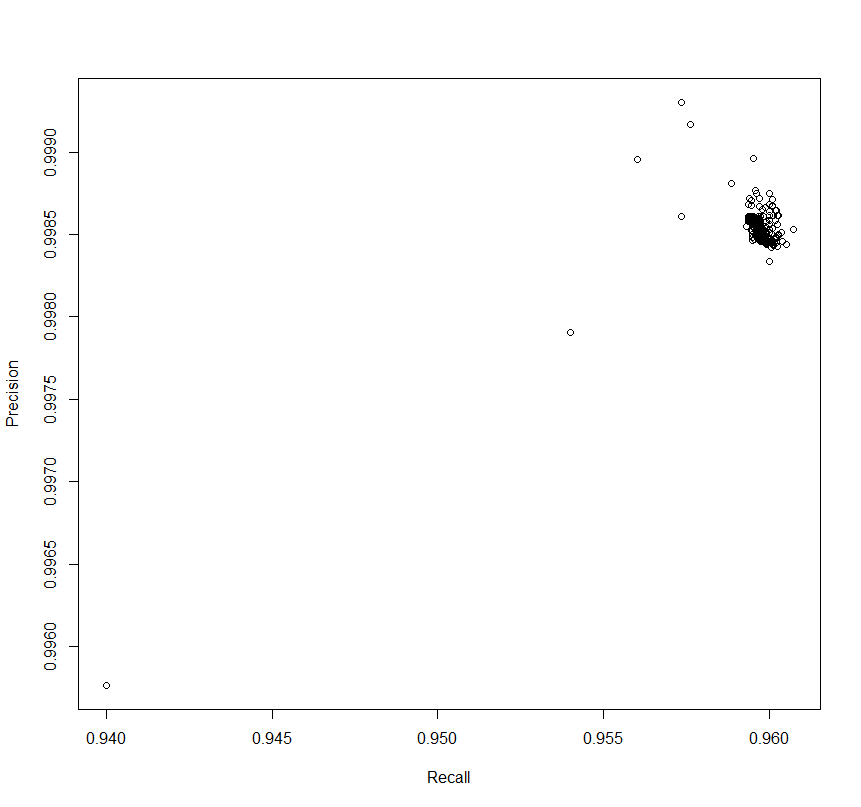
\includegraphics[scale=0.7]{./PerceptronSet1.png}
\end{center}
\caption{Precision Recall Curve of Set 1(in red).}
\label{Img:PrecisionRecallS1}
\end{figure}

\section{Exercise 1.4: Classification into more than two classes}
\begin{enumeration}
\item On option could be, to train for $n$ classes $n$ ANN's: Every ANN classifies if the input is in class $n$ or not. -TODO \\
\item ANother option are $2^n$ classifiers, one for every pair of classes. -TODO

\end{enumeration}


\end{document}
